% research question:
% how does each hyperparamter play a part in evolutionary decision tree performance?
% ^ maybe too abstract
% how does an gdt compare with other data classification algorithms of similar nature
% more broad like:
%   to what extent can a genetic algorithm be used to optimize decision trees for data classification

% TODO: Change font to helvetica
% double spacing

% latex template
\documentclass[12pt]{article}
\usepackage[utf8]{inputenc}
\usepackage[english]{babel}
\usepackage[margin=1in]{geometry}
\usepackage{caption} % figure captioning
\usepackage{amsmath} % equation tools
\usepackage{amssymb} % math symbols
\usepackage{mathtools} % math rendering improvements
%\usepackage{siunitx} % standard units
\usepackage{graphicx} % add images
%\usepackage{wrapfig} % position images
\usepackage{float} % position images pt.2
%\usepackage[makeroom]{cancel} % cross out text
%\usepackage[version=4]{mhchem} % chemical equations
%\usepackage{multicol} % multiple columns
%\usepackage{pgfplots} % built in plotter
%\pgfplotsset{width=10cm,compat=1.9} % plotter settings
\usepackage{hyperref} % table of contents links
\usepackage{indentfirst} % indent first paragraph after section

\hypersetup{
    colorlinks,
    citecolor=black,
    filecolor=black,
    linkcolor=black,
    urlcolor=black
}

\renewcommand{\baselinestretch}{1.5} % line spacing
\newcommand{\fline}{\par\noindent\rule{\textwidth}{0.1pt}} % horizontal line (wide)

\title{EE TITLE}
\author{Bryan Deng}
\date{}

\begin{document}

\maketitle
\newpage
\tableofcontents
\newpage

\section{Background Information}

\subsection{Machine Learning and its Applications}

Machine learning (ML) is a branch of artificial intelligence that uses large datasets and algorithms to mimic the way humans learn and improve accuracy over time \cite{what_is_ml_ibm}. Since its debut in 1952, it has been steadily gaining popularity for its abilities in recognizing patterns and continuous learning. Machine learning powers many of the applications we use on a daily basis, including chatbots, language translation tools, and social media feeds \cite{what_is_ml_mit}.

Where machine learning shines is in its ability to solve problems that would typically be either impossible for impractical for traditional algorithms. Furthermore, machine learning models are able to generalize these solutions and apply them to additional problems it has never encountered before.

In short, machine learning is a combination of computer science, statistics, and optimization. It uses knowledge from different fields to ``teach'' computers to complete tasks. As the model looks at more and more data, it starts to recognize patterns among it and optimizes itself. The main problem that data scientists are trying to solve with regard to machine learning is how we actually optimize the algorithms.

\subsection{Decision Trees}

When most think about machine learning, the first thing that comes to mind are neural networks. Neural networks, which are complex yet powerful algorithms, only make up one branch of machine learning itself, called deep learning. Deep learning has built a reputation to be extremely versatile and powerful, able to generalize any function across data. However, one of its biggest drawbacks is that the with the limits of our current technology and understanding of deep learning, neural networks are often described as a ``black box'' \cite{Buhrmester_Munch_Arens_2019}. In other words, all we know is to give the network a set of inputs and outputs, and we have very little understanding of its inner behavior or the interactions between neurons.

There exists another branch of machine learning, called supervised learning. This approach aims to solve problems of data classification and regression \cite{Supervised_unsupervised_learning}. The data that is deals with is still made of inputs and outputs. Each characteristic of the data is called a \textit{feature} and the outputs are called \textit{labels}. One of the most well established models within supervised learning is the decision tree. They are binary trees which employ a straightforward \textit{if-else} flow to classify or regress data. Contrary to neural networks, decision trees are much easier to interpret for humans. This paper will focus on data classification rather than regression with decision trees.

Binary trees are made up of nodes, which are connected by edges. As its name suggests, each node is connected to two child nodes, which have their own respective child nodes, etc. Nodes at the bottom of the tree are called leaves, and do not branch out to any more children.

\begin{figure}[H]
    \centering
    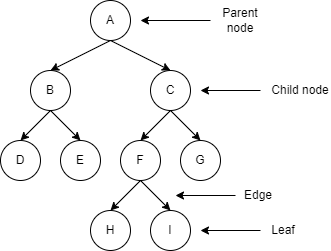
\includegraphics[scale=0.6]{figs/binary_tree.png}
    \caption{Binary Tree Diagram}
    \label{fig:binarytree}
\end{figure}

Decision trees use the structure of binary trees to classify data. Non-leaf nodes are referred to as ``split nodes''. Split nodes each have a feature and a split value. When data reaches that node, it is passed on to the left child if the feature value is less than the split value, and to the right child if otherwise. In dealing with categorical features, such as color, they are each mapped to an integer, so they can be treated the same as numerical features. Leaf nodes each contain a label. If data reaches a leaf node, it is classified as that label.

\begin{figure}[H]
    \centering
    \fbox{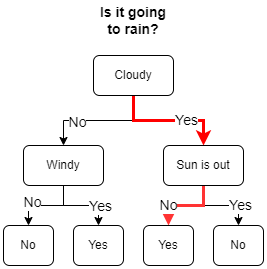
\includegraphics[scale=0.7]{figs/decision_tree.png}}
    \caption{Decision Tree Diagram}
    \label{fig:decisiontree}
\end{figure}

\hyperref[fig:decisiontree]{Figure 1} shows a simple decision tree to predict whether it will rain based on other weather conditions. Given a cloudy day with no sun, the model will predict that it will rain, as outlined by the red lines on the diagram.

The standard way to generate a decision tree is to use a top-down greedy recursive algorithm based on how many values are incorrectly classified, or gini-impurity. At each step of the tree, the split value is determined by testing out every single value of every single feature, and seeing which one yields the lowest gini-impurity. The left child of the current node is then built using the data that falls under the split value, and the right child is built using the remaining data. This process continues until the gini-impurity is less than a preset value, or until a certain depth is reached. Certain algorithms for decision tree generation also balance the binary tree for reduced time complexity in testing \cite{dt_skl_doc}.

\subsection{Genetic Algorithm}

Taking a page straight out of Darwin's theory of evolution, genetic algorithms employ the principle of ``survival of the fittest''. Biological evolution has been able to produce billions \cite{Sweetlove_2011} of different species of organisms that have all become very well adapted to their environments. It does so by ensuring that only the individuals that are able to survive in their environments the best are able to reproduce. Those that are unable to find food, get hunted easily by predators, or easily catch diseases are unable to pass on their genes to the next generation. This also ensures that only the strongest genes are kept from generation to generation.

Furthermore, evolution maintains diversity within species to ensure robustness and the potential to introduce new strengths. This is done through mutations, where certain values of an individual's DNA sequence are changed, thereby altering their appearance or behavior. The mutations that turn out to be beneficial can help the species in their specific environments. An example of mutations can be found in different species of snakes. Both cobras and vipers evolved from the same ancestor. However, venom from cobras attack the target's nervous system while that from the viper attacks the cardiovascular system.

It is through the combination of the principle of ``survival of the fittest'' promoting diversity that biological evolution has produced so many species of organisms that are each so well adapted to their environments. In short, evolution is very well versed in solving a complex optimization problem.

There exist certain computational problems that would take an unrealistic amount of computational resources to optimize by brute force, or where there lies no straightforward path to a solution. The genetic algorithm aims to mimic biological evolution as close as possible, seeing the potential for optimizing and solve such problems. It is composed of six main steps: initialization, fitness evaluation, selection, crossover, mutation, and finally termination. Each step of this process aims to mimic one part of what makes biological evolution so effective and robust.

Initialization randomly produces the first generation of individuals. In the genetic algorithm, each individual represents one possible solution to the final problem. These are usually represented in the form of a data structure. Each individual data structure is composed of many smaller pieces of data, which are analogous to the genes of a biological organism. Together, the data determine the actions of the individual. The first generation is not expected to perform well, as all the data was generated from a random number generator.

Fitness evaluation if the first step of the actual evolving or optimization process. Each individual has their fitness assessed based on a set of criteria. Fitness is represented by a single number, which can be determined by factors like performance, accuracy, or speed of the individual. The fitness value given to each individual is to encourage better performing genes into being passed onto the next generation, and vice versa.

As ``survival of the fittest'' suggests, the selection step picks the best individuals based on fitness to pass their genes onto the next generation. However, in order to maintain diversity, this step is not as simple as just sorting the individuals by fitness and picking the best ones for reproduction. Returning to the principle of diversity, there may be certain genes in the less fit individuals that can be beneficial in certain cases, so it is important that we do not entirely wipe them out. At the same time, those with higher fitness are more likely to contain more useful genes. Therefore, selection is randomized, with the probability of each individual being selected being weighted based on their fitness. This balances survival of the fittest and diversity.

Crossover is analogous to reproduction. As with its biological counterpart, crossover can be either sexual or asexual. For sexual crossover, two parent individuals are needed. A child is produced by taking a subset of genes from the first parent, and a subset of genes from the other parent. For asexual crossover, only one parent is needed. A child is produced by swapping specific or a subset of genes' order. After crossover, the child individual has traits of both its parents, and its unique combination of genes can possibly explore further into the solution space.

Mutation is what maintains diversity in the population. This introduces possible new genes into the population pool, or possibly new combinations of genes as well. Each individual has a random chance to be selected for mutation. In mutation, a random gene is chosen, and its value is altered. This is the last step of the optimization process.

The steps from fitness evaluation to mutation are repeated over a predetermined number of generations, or until a stopping criterion is reached. This last step is called termination, which determines when the main loop is to end.

\section{Genetic Decision Tree}

The genetic algorithm brings many benefits to the optimization of abstract problems. An abstract problem with infinite possible solutions is decision tree construction and structure. There is a potential to use the genetic algorithm to construct and optimize decision trees. For the purpose of this paper, this method will be coined the ``Genetic Decision Tree''.

A Genetic Decision Tree (GDT) uses a genetic algorithm to optimize decision trees. It aims to take the benefits from both decision tree classifiers and random forests, while adding a layer of the genetic algorithm that increases its accuracy with training.

From decision trees, the GDT takes the ability to generate a singular, human interpretable tree as its final model. This can be useful in analysis, hyperparameter tweaking, or presentation. And from random forests, it introduces a layer of randomness, which will be further harnessed by the genetic algorithm. This allows the model to explore a larger solution space, and minimize the chance of fitting into a suboptimal solution. In short, the GDT fitting algorithm aims to combine the benefits of randomness in a random forest into a singular, or smaller subset of optimized decision trees.

\begin{figure}[H]
    \centering
    \fbox{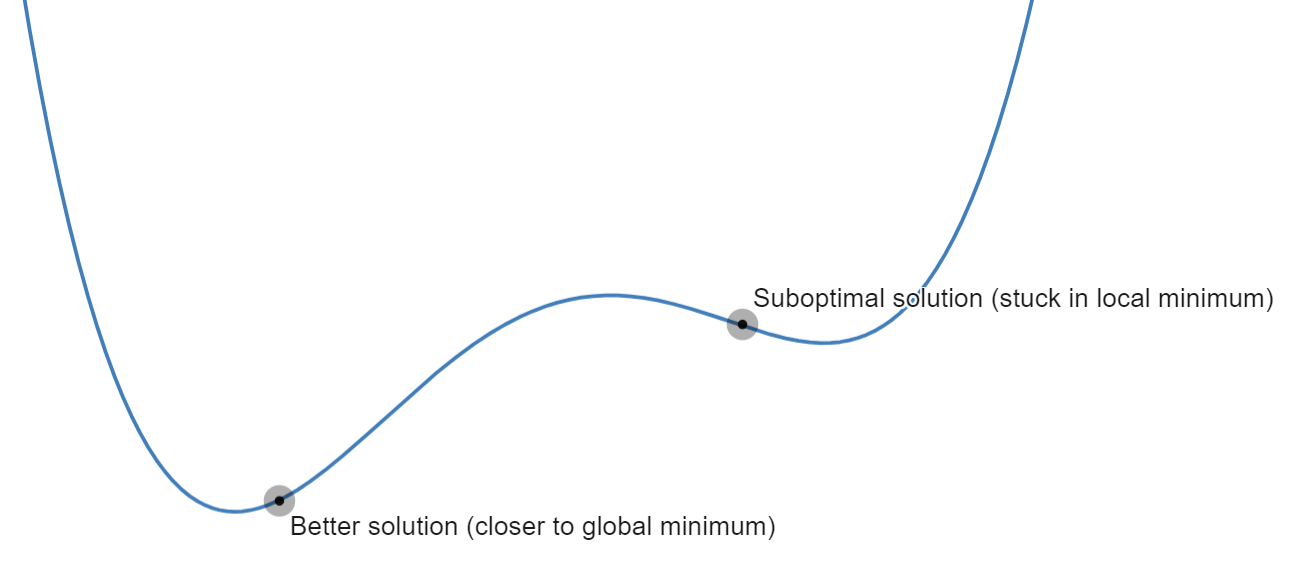
\includegraphics[scale=0.5]{figs/solution_space.png}}
    \caption{The solution space, represented by the curve (lower is better).}
    \label{fig:solutionspace}
\end{figure}

The GDT will be implemented in the Python3 programming language.

\subsection{Initialization}

The GDT population is composed of $n$ randomly generated decision trees, where $n$ is the population size. A randomly generated tree starts with a root node. Each of its children is then either a split node or a leaf node, determined by a probability $p$. If a node is assigned as a split node, it is randomly assigned a feature and a corresponding split value. Otherwise, if it is a leaf, it is randomly assigned a label. Further restrictions are put in place to ensure that no branch of the tree can only lead to a single label. This step is repeated until a desired depth is reached, or until all branches end in leaf nodes \cite{faik_2020}. Unlike a normal decision tree, there is no maximum depth with each individual in the GDT population. This is due to the fact that the depth may grow in crossover. Rather, they will all be generated up to an \textit{optimal} depth to begin.

\subsection{Fitness Evaluation}

The fitness for each individual in the population will be measured by the following formula \cite{faik_2020}:

\[ F_i = c_1 \cdot a_i - c_2 \cdot (d_i - d_\text{opt})^2 \]

\begin{itemize}
    \item $F_i$ is the fitness of the $i$-th individual.
    \item $a_i$ is the accuracy of the $i$-th individual on the training data.
    \item $d_i$ is the depth of the $i$-th individual.
    \item $d_\text{opt}$ is the optimal depth of the tree.
    \item $c_1, c_2$ are predetermined constants.
\end{itemize}

The depth of each individual is extremely important. Trees that are smaller than the optimal depth may yield suboptimal results. Those that are bigger may be detrimental to performance and time complexity, especially if they reproduce and make even larger trees in future generations. Therefore, the function $(d_i - d_\text{opt})^2$ has been specially chosen to encourage the optimal depth. It is an upwards opening parabola with a minimum when $d_i = d_\text{opt}$, which increases on either side. A value is subtracted from an individual's fitness depending on its depth. Trees that are either too big or small are punished with a decrease in fitness, and therefore have a lesser chance of being selected for the next generation.

The values of $c_1$ and $c_2$ are hyperparameters which can be adjusted according to performance of the algorithm in testing.

\subsection{Selection}

The selection process will be a combination of two separate algorithms. The first of which will be tournament selection. A random set of $k$ individuals will be ranked by fitness, and the highest score will be able to move on to the crossover stage. This process is repeated twice, once for each parent in crossover. The random nature of this selection process ensures that diversity is maintained between generations, and that certain traits will not be entirely lost \cite{blickle_1997}.

The second selection process will be elitism. This is where the fittest individuals from the previous generation will be moved directly on to the current generation, without crossover. This is to ensure that the traits of the best individuals from the previous generation are not lost in selection or crossover.

A total of $t$ individuals will be moved onto the next generation through elitism. The remaining $n - t$ spots will be filled through tournament selection and crossover.

\subsection{Crossover}

For crossover, two parent trees will produce two child trees in order to maintain the population count. The first child will originally be a direct copy of the first parent. A random node is then selected from each parent. The node from the first parent, and its entire subtree, will be replaced by the node from the second parent and its subtree. The same process will be repeated for the second child, except with the roles of the parents reversed.

\begin{figure}[H]
    \centering
    \fbox{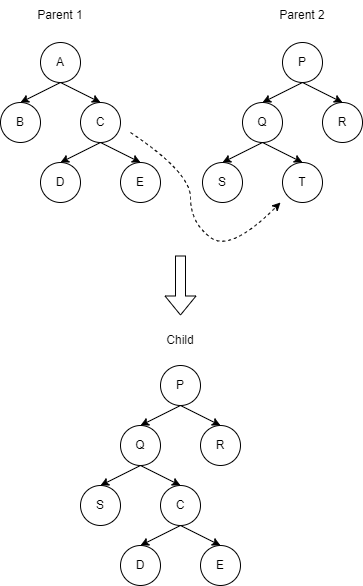
\includegraphics[scale=0.5]{figs/tree_crossover.png}}
    \caption{Decision tree crossover}
    \label{fig:treecrossover}
\end{figure}

\subsection{Mutation}

If a tree is chosen for mutation, it will have one of its value's traits randomly chosen and altered. If the node selected is a split node, its feature and split value will be randomly altered. Otherwise, if the node selected is a leaf node, it will have its label randomly altered. Precautions will be put in place to make sure that each subtree can still lead to more than one label.

\subsection{Termination}

There are two conditions for termination. The first of which is when the number of generations has reached a predetermined $n$. The other condition is when the average fitness does not improve by a predetermined threshold for $x$ generations. Which ever condition comes first is when the GDT will terminate.

\section{Experimental Analysis}

The performance of the GDT will be evaluated on three main factors: training speed, training convergence, and testing accuracy. The hyperparameters of the GDT will be altered in order to see what effect each one has on the performance factors of the algorithm. Each test with its specific parameters will be run three times. Each iteration will have a different but controlled random seed, in order to minimize the chances of a fluke.

%! maybe run in ipython with jupyter
All the tests will be run on an AMD Ryzen 7 4700U and CPython 3.8.10.

\subsection{Population Size}

\subsection{Crossover Probability}

\subsection{Selection Constants}

\subsection{Selection Methods}

\subsection{Mutation Probability}

\subsection{Generation Count}

\bibliographystyle{plain}
\bibliography{refs}

\end{document}

